% !TEX root = ../HDR.tex
%%%%%%%%%%%%%%%%%%%%%%%%%%%%%%%%%%%%%%%%%%%%%%%%%%%%%%%%%%%%%%%%%%%%%%%%%%%%%%%%%%
\chapter{Architecture de schéma spatio-séquentielle}

\noindent
Pour permettre l'organisation intelligente des comportements d'un agent interagissant avec un environnement spatial, tel qu'un robot dans le monde physique, les comportements ne doivent pas seulement s'organiser dans le temps mais aussi dans l'espace. 

\emph{Un mécanisme de schéma est un mécanisme capable de créer et réitérer des comportements hiérarchiques spatio-séquentiels sur la base de préférences interactionnelles initiales. }


Ron Sun réutilise la notion de \og \an{representational redescription} \fg\ proposée par Annette Karmiloff-Smith \cite{karmiloff-smith_meta-processes_1986}.

\an{Here I take the more ``eclectic'' proposition that acknowledge representation is important while maintaining that it is mediated by direct comportement} \cite[p.~10]{sun_symbol_2000}

\section{Inférence de la structure spatiale}

L'article ``\an{Autonomous construction and exploitation of a spatial memory by a self-motivated agent}'' \cite{gay_autonomous_2017} présente comment l'agent peut inférer la structure de l'espace à partir de ses expériences d'interaction.


\section{Spatial Enactive Decision Process (SEDP)}
\label{sec:sedp}

Le Spatial Enactive Decision Process (SEDP) étend le Enactive Decision Process introduit en section \ref{sec:edp} en ajoutant des propriétés spatiales à l'outcome: une position et un déplacement.

\begin{figure}[ht]
	\centering
	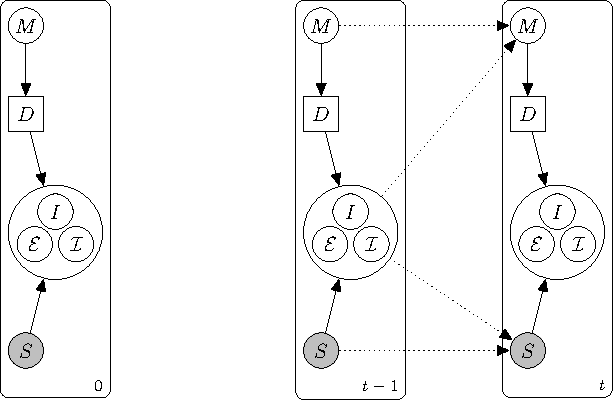
\includegraphics[width=0.6\textwidth]{Figures/5_sedp.pdf}
	\caption{Spatial Enactive Decision process (\cite{georgeon_artificial_2024}, Fig. 5) }
	\label{fig:sedp}
\end{figure}


\section{Ontologie basée sur les affordances}

Renvoie à la notion de bundle introduite dans la Section \ref{sec:pragmatisme} sur l'épistémologie pragmatique.

\section{Enactive Cognitive Architecture (ECA)}

\begin{figure}[ht]
	\centering
	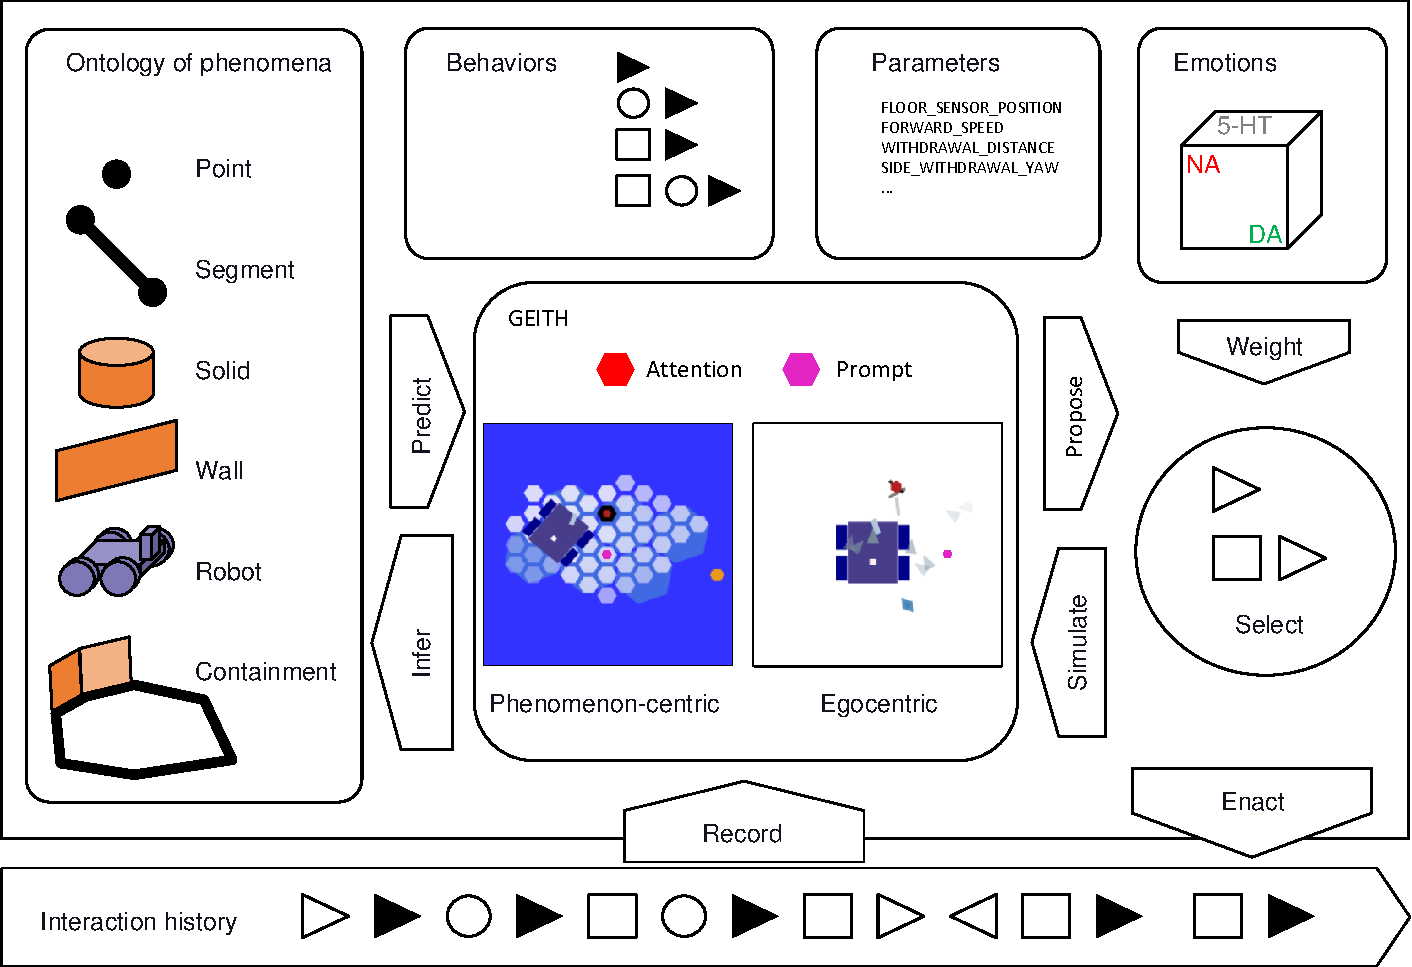
\includegraphics[width=0.6\textwidth]{Figures/5_ECA.pdf}
	\caption{The Enactive Cognitive Architecture (ECA) depuis \cite{georgeon_reducing_2024}}
	\label{fig:ECA}
\end{figure}

La Figure \ref{fig:ECA} montre la Enactive Cognitive Architecture décrite dans \cite{georgeon_reducing_2024}




\section{Simulation interne}

Game Engine in The Head

\section{Explicabilité et inference causale}

\subsection{Expérimentation de l'abeille}

\noindent
Cette expérimentation examine comment générer des comportements plus sophistiqués sur la base des mécanismes instinctifs simulés dans l'expérimentation de la limule présentée en Section~\ref{sec:horseshoe}.
Dans cette expérimentation appelée \emph{expérimentation de l'abeille}, nous avons étendu les mécanismes perceptifs et motivationnels d'ECA, et ajouté un \emph{mécanisme attentionnel}.

Le mécanisme attentionnel sélectionne une cible particulière parmi les cibles présentes dans le champ visuel en fonction d'une valence associée au \an{bundle} représentant ce type de cible.
Une fois l'attention portée sur une cible donnée, des mécanismes identiques à ceux de l'expérimentation de la limule conduisent l'abeille à s'en rapprocher.

L'abeille dispose des mêmes types d'interactions avec une cible que la limule, construites à partir des décisions \texttt{move forward} , \texttt{turn left} et \texttt{turn right}, et les \an{inputs} \texttt{increase left}, \texttt{increase front}, \texttt{increase right}, \texttt{decrease}, \texttt{stable}.  
L'interaction \interaction{move forward, eat} est enactée quand 

Le mécanisme perceptif visuel a été étendu par l'ajout d'une observation représentationnelle en parallèle aux événements d'interaction. 

appelé \emph{canal perceptif statique}, en parallèle au canal précédent que nous désignons maintenant par le terme de \emph{canal perceptif dynamique}.
Le canal perceptif statique mémorise une représentation iconique de chaque cible qui permet de la reconnaitre, ainsi qu'une indication du temps écoulée depuis la dernière visite de cette cible. 

L'article \an{Early-stage vision of composite scenes for spatial learning and navigation} \cite{georgeon_early-stage_2011} rapporte un exemple de comportements que nous avons pu générer avec ce mécanisme.
Cette expérimentation, illustrée en Figure \ref{fig:bee}, s'inspire des comportements de butinage des abeilles. 
Certaines cibles représentent des fleurs qui peuvent être butinées. 
La ruche permet de dépôt de pollen.
D'autres cibles peuvent simplement servir de \an{landmarks} qui l'abeille peut utiliser pour retrouver son chemin en direction d'un champ de fleurs puis pour retourner à la ruche.   

Lorsque l'abeille arrive sur une fleur, elle découvre que cette fleur peut être butinée et associe cette information à la représentation iconique de cette fleur apprise par le système perceptif statique. 
De même, l'abeille associe l'interaction de \og dépôt de pollen \fg\ à la ruche. 

Le nouveau système motivationnel associe une valence motivationnelle à chaque cible en fonction des interactions qu'elles permettent et de l'état courant de l'abeille. 
Au début, l'abeille apprend à se diriger vers les cibles de la même façon que dans l'expérimentation précédente. 
Lorsqu'elle arrive sur une cible, elle associe l'interaction permise par cette cible à la représentation iconique de cette cible: le fait que les fleurs peuvent être butinées et que la ruche permet le dépôt de pollen. 
Ces valences motivationnelles sont propagées sur les autres cibles en fonction de leur temps de trajet estimé par rapport aux fleurs ou à la ruche. 
Lorsque l'abeille est en phase de recherche de pollen, la cible qui est la plus proche du champ de fleur reçoit sont attention, et l'abeille navigue ainsi de cibles en cibles jusqu'a retrouver le champ de fleurs. 
Le même mécanisme est utilisé pour retrouver la ruche quand l'abeille porte du pollen. 
La vidéo présente un exemple de comportement obtenu \cite{georgeon_bee_2011}. 

\begin{figure}[ht]
	\centering
	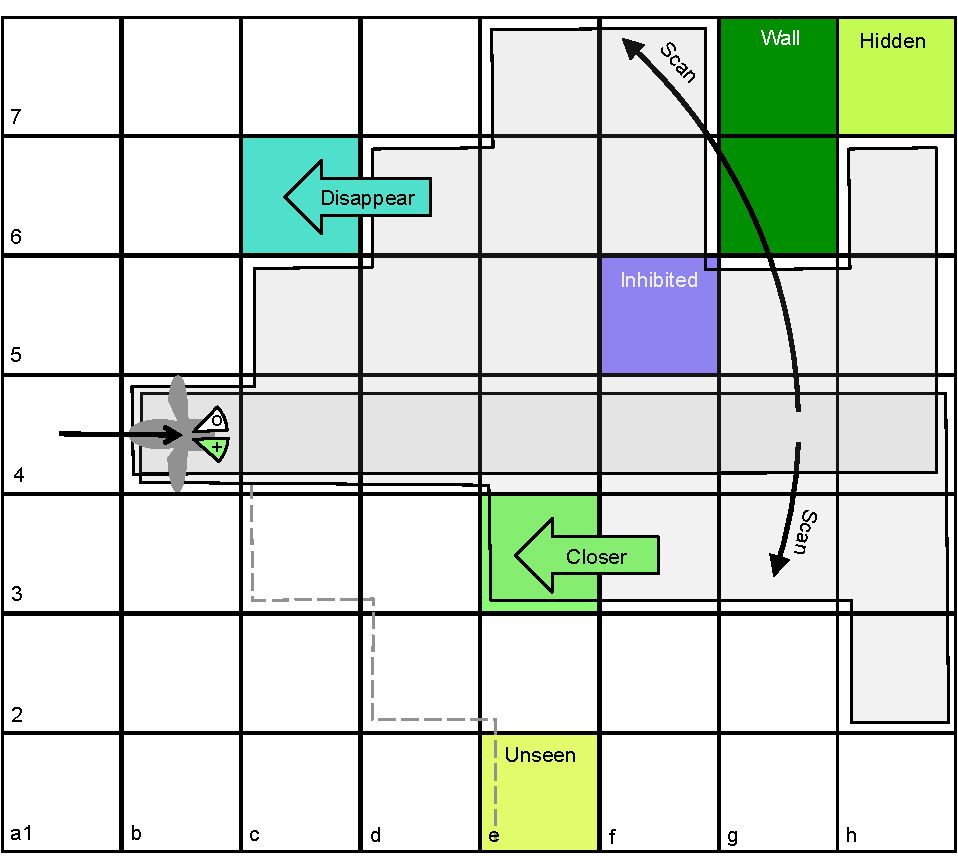
\includegraphics[width=0.6\textwidth]{Figures/4_bee.pdf}
	\caption{
		% Système visuel implémenté dans la \an{Bee experiment} (\cite{georgeon_early-stage_2011}, Fig. 3). 
		Expérimentation de navigation dans une scène variée. 
		Cellule violette (e5): la ruche. Cellules bleues: fleurs. 
		Cellules vert-foncé: murs que l'abeille ne peut pas traverser et qui masquent le champ visuel. 
		Autres cellules colorées: \an{landmarks} que l'abeille peut utiliser pour naviguer.   
	}
	\label{fig:bee}
\end{figure}

